\documentclass[openbib]{article}

\usepackage{color}
\usepackage{ctex}
\usepackage{mathtools}
\usepackage{amsmath}
\usepackage{graphicx,psfrag,epsfig}
% Copyright 20120 Liutao Tian, MIT License
% https://github.com/andy123t/code-latex-style/

\usepackage{listings,color}

% Matlab highlight color settings
%\definecolor{mBasic}{RGB}{248,248,242}       % default
\definecolor{mKeyword}{RGB}{0,0,255}          % bule
\definecolor{mString}{RGB}{160,32,240}        % purple
\definecolor{mComment}{RGB}{34,139,34}        % green
\definecolor{mBackground}{RGB}{245,245,245}   % lightgrey
\definecolor{mNumber}{RGB}{134,145,148}       % gray

\definecolor{Numberbg}{RGB}{237,240,241}     % lightgrey

% Python highlight color settings
%\definecolor{pBasic}{RGB}{248, 248, 242}     % default
\definecolor{pKeyword}{RGB}{228,0,128}        % magenta
\definecolor{pString}{RGB}{148,0,209}         % purple
\definecolor{pComment}{RGB}{117,113,94}       % gray
\definecolor{pIdentifier}{RGB}{166, 226, 46}  %
\definecolor{pBackground}{RGB}{245,245,245}   % lightgrey
\definecolor{pNumber}{RGB}{134,145,148}       % gray

\lstnewenvironment{Python}[1]{
	\lstset{language=python,               % choose the language of the code
		xleftmargin=30pt,
		xrightmargin=10pt,
		frame=l,
		framesep=15pt,%framerule=0pt,  % sets the frame style
		%frame=shadowbox,rulesepcolor=\color{red!20!green!20!blue!20},
		%basicstyle=\small\ttfamily,          % sets font style for the code
		basicstyle=\footnotesize\fontspec{Consolas},
		keywordstyle=\color{pKeyword},       % sets color for keywords
		stringstyle=\color{pString},         % sets color for strings
		commentstyle=\color{pComment},       % sets color for comments
		backgroundcolor=\color{pBackground}, % choose the background color
		title=#1,                            %\lstname show the filename of files
		emph={format_string,eff_ana_bf,permute,eff_ana_btr},
		emphstyle=\color{pIdentifier}
		showspaces=false,                    % show spaces adding particular underscores
		showstringspaces=false,              % underline spaces within strings
		showtabs=false,                      % show tabs within strings adding particular underscores
		tabsize=4,                           % sets default tabsize to 2 spaces
		captionpos=t,                        % sets the caption-position to bottom
		breaklines=true,                     % sets automatic line breaking
		framexleftmargin=5pt,
		fillcolor=\color{Numberbg},
		rulecolor=\color{Numberbg},
		numberstyle=\tiny\color{pNumber},
		numbersep=9pt,                      % how far the line-numbers are from the code
		numbers=left,                        % where to put the line-numbers
		stepnumber=1,                        % the step between two line-numbers.
}}{}

\lstnewenvironment{Python1}[1]{
\lstset{language=python,               % choose the language of the code
  xleftmargin=30pt,
  xrightmargin=10pt,
  frame=l,
  framesep=15pt,%framerule=0pt,  % sets the frame style
  %frame=shadowbox,rulesepcolor=\color{red!20!green!20!blue!20},
  %basicstyle=\small\ttfamily,          % sets font style for the code
  basicstyle=\footnotesize\fontspec{Consolas},
  keywordstyle=\color{pKeyword},       % sets color for keywords
  stringstyle=\color{pString},         % sets color for strings
  commentstyle=\color{pComment},       % sets color for comments
  backgroundcolor=\color{pBackground}, % choose the background color
  title=#1,                            %\lstname show the filename of files
  emph={format_string,eff_ana_bf,permute,eff_ana_btr},
  emphstyle=\color{pIdentifier}
  showspaces=false,                    % show spaces adding particular underscores
  showstringspaces=false,              % underline spaces within strings
  showtabs=false,                      % show tabs within strings adding particular underscores
  tabsize=4,                           % sets default tabsize to 2 spaces
  captionpos=t,                        % sets the caption-position to bottom
  breaklines=true,                     % sets automatic line breaking
  framexleftmargin=5pt,
  fillcolor=\color{Numberbg},
  rulecolor=\color{Numberbg},
  numberstyle=\tiny\color{pNumber},
  numbersep=9pt,                      % how far the line-numbers are from the code
  numbers=left,                        % where to put the line-numbers
  stepnumber=1,                        % the step between two line-numbers.
}}{}



\usepackage{fontspec}
\usepackage{bm}
\graphicspath{{figures/}}
\renewcommand{\contentsname}{\centerline{目录}}

\usepackage{multirow}
\begin{document}
	\title{深度学习基础}  %  https://zhuanlan.zhihu.com/p/60574682
	
	\maketitle
	
	\newpage
	\tableofcontents
	\newpage
	
\section{深度学习发展阶段}
早期绝大多数机器学习与信号处理技术都使用浅层结构,一般含有一到两层非线性特征变换。常见包括:支持向量机,高斯混合模型,条件随机场,逻辑回归。在解决大多数简单问题或有较多限制条件的问题上效果明显,无法处理复杂问题。

深度学习(deep learning)通过其他较简单的表示来表达复杂表示,解决了表示学习中的核心问题。具体来说,它是机器学习的一种,一种能够使计算机系统从经验和数据中得到提高的技术。

一般来说,目前为止深度学习已经经历了三次发展浪潮:20 世纪40 年代到 60 年代深度学习的雏形出现在 控制论(cybernetics)中,20 世纪 80 年代到90 年代深度学习表现为 联结主义(connectionism),直到 2006 年,才真正以深度学习之名复兴。

20世纪40年代初,Warren Maculloach和Walter Pitts在分析和总结了生物神经元的基本结构后,设计了M-P神经元模型,并指出其运行简单逻辑运算的机制。

20世纪40年代末,Donald Hebbian在生物神经可塑性机制的基础上提出了一种无监督学习规则,称为Hebbian学习。同期Alan Turing的论文中描述了一种“B型图灵机”。之后,研究人员将Hebbian学习的思想应用到“B型图灵机”上。

1958年,Rosenblatt提出感知机(Perception)————可以模拟人类感知能力的神经网络模型。并提出了一种接近于人类学习过程的学习算法,通过迭代,试错使得模型逼近正解。

1969年,Minsky和Papert指出感知机网络的两个关键性缺陷:无法处理异或回路;计算资源制约了大型神经网络所需要的计算。

1975年,Werbos博士在论文中发表了反向传播算法,使得训练多层神经网络模型成为现实。

1983年,John Hopfield提出一种用于联想记忆和优化计算的神经网络,称为Hopfield网络,在旅行商问题上获得突破。

1984年,Geoffrey Hinton提出一种随机化版本的Hopfield网络————玻尔兹曼机。

1989年,Yann Lecun将反向传播算法应用到卷积神经网络,用于识别邮政写手数字并投入真实应用。

20世纪末期,Vapnik基于统计学习理论提出了支持向量机(Support Vector Machine,SVM),通过核(kernel)技巧把非线性问题转换成线性问题。

2006年,Hinton等人提出限制玻尔兹曼机(Restricted Boltzmann Machine)通过非监督学习的方式建模神经网络的结构,再由反向传播算法学习网络内部的参数,使用逐层预训练的方法提取数据的高维特征。

随着计算机硬件能力的提高,特别是图像处理器(Graphics Processing Unit,GPU)强大的并行计算能力非常适合神经网络运行时的矩阵运算。随着神经网络层数的不断加深,Hinton等人重新将不断变深的神经网络重新定义为深度学习。

\section{感知机}
感知机算法时由Frank Rosenblatt提出,由此揭开了人工神经网络研究的序幕。
\subsection{感知机的起源}

\begin{figure}[htbp]
	\centering
	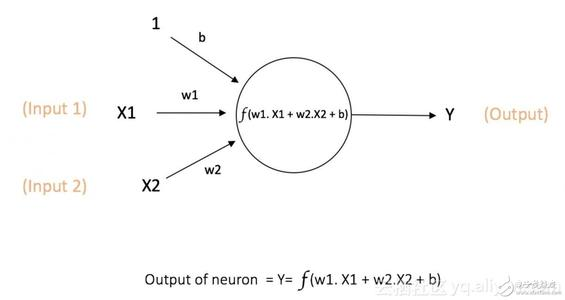
\includegraphics[scale=0.4]{感知机}
\end{figure}

图中$x_1,x_2$代表人们选择的输入信号(input),y为输出信号(output),$w_1,w_2,b$为感知机内部的参数,称为权重(weight)。

Perceptron 简单的单层线形二进制分类器。接收输入和与其相连的权重(表示输出变量的相对重要性),将它们结合起来产生输出。输出接下来被用于分类。只要被处理的数据线性可分,就能使用感知机模型不断地进行模型训练和参数优化,最后得到一个能够对数据进行二分类的模型。
	
数学表达式:$$f(x) = sign(w\bullet x + b)== \left\{ \begin{array}{cl}
		+1 & : \ w\bullet x + b> 0 \\
		-1 & : \  w\bullet x + b< 0
	\end{array} \right.$$
	
输出结果值-1和1就可以被看作数据经过模型计算后输出的对应标签。如果处于二维空间中,那么$w\bullet x + b=0$对应的就是输入数据进行二分类的那条直线,也叫作分割超平面(Separating Hyperplane)。
	
感知机的多个输入信号都有各自的权重,权重越大,对应信号的重要性就越高。我们能设置不同的权重和偏置值来让感知机实现不同的功能。也可以设计学习算法,使得计算机能够自动地调整感知地权重和偏置,而不需要人的直接干预。
	
优点:很容易地处理线性可分问题。缺点:不能处理非线性问题。故就出现了能够处理非线性问题的多层感知机模型
	
一个多层感知机(MLP)由几个含有全连接层的感知机组成,在感知机的输入层(Input Layer)和输出层(Output Layer)之间加入了新的网络层次:隐藏层(Hidden Layer)形成一个简单的前馈神经网络。多层感知机具备一种后向传播能力。
	
\subsection{感知机的局限性}
一方面是这类算法只能处理线性可分的问题,即只能表示由一条直线分割额空间。对于线性不可分的问题,如异或门,没有可行解。

感知机需要人工选择特定的特征作为输入,极大限制了感知机的应用,故要设置自动提取复杂的特征。
\section{前馈神经网络}
联结主义(connectionism)或并行分布处理 ( parallel distributed processing):当网络将大量简单的计算单元连接在一起时可以实现智能行为。这种见解
同样适用于生物神经系统中的神经元,因为它和计算模型中隐藏单元起着类似的作用

解决感知机困境的方法就是将感知机堆叠,进而形成多层神经网络,也称深度神经网络(Deep Neural Network,DNN)。

1975年,Werbos博士在其论文中证明将多层感知机堆叠成神经网络,并利用反向传播算法训练神经网络自动学习参数,解决"异或门"。

\begin{figure}[htbp]
	\centering
	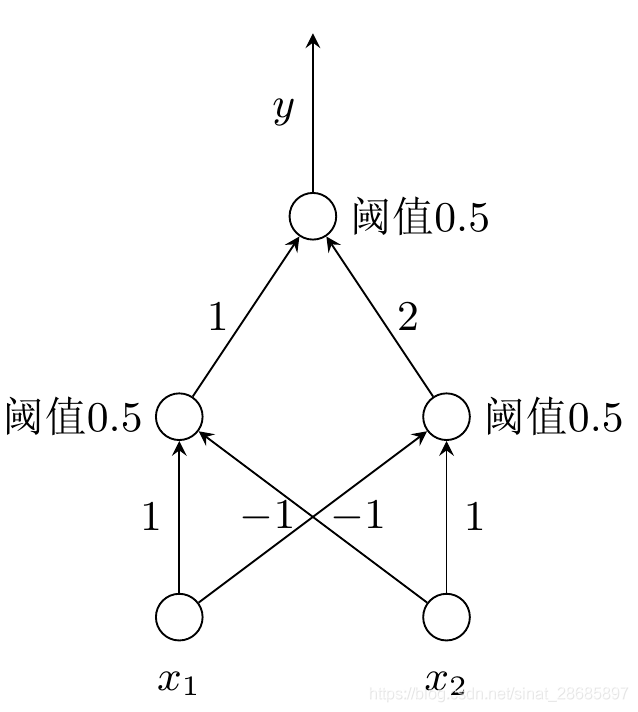
\includegraphics[scale=0.2]{多层感知机异或门}
\end{figure}

使用三个简单感知机组成一个两层的感知机,满足异或门响应条件。

虽然多层神经网络的出现解决了感知机的问题,但是相比较于同时期的 支持向量机算法,多层神经网络缺乏完备的数学理论证明。

分布式表示(distributed representation):系统的每一个输入都应该由多个特征表示,并且每一个特征都应该参与到多个可能输入的表示。
\subsection{神经元}
神经元(Neuron)是构成神经网络的基本单元,其主要是模拟生物神经元的结构和特性,接受一组输入信号并产生输出。

McCulloch和Pitts根据生物神经元的结构,将一种简单的人工神经元模型逐渐发展为现代人工神经元模型。
\begin{figure}[htbp]
	\centering
	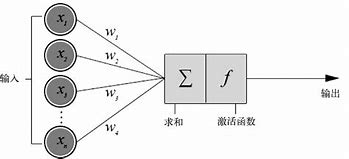
\includegraphics[scale=0.5]{人工神经元}
\end{figure}

在引入函数f(x)后,感知机就可以写成神经元的形式,输入信号会被f(x)转换,转换后的值就是输出y,这种将输入信号的总和转换为输出信号的函数称为激活函数(Activation Funcation)

\subsection{激活函数}
了解感知机后,可得到一个增加偏置的单层神经网络模型的数学表示:$f(x)=W \bullet X+b$。增加偏置是能够使模型具有更强的变换能力,在面对不同的数据时拥有更好的泛化能力。上诉模型为线性模型,对非线性问题存在很大的局限性。激活函数一般是非线性的,为神经网络引入了非线性因素,这样才能更逼近更复杂的数据分布。激活函数也限制了输出的范围,控制该神经元是否激活。激活函数提升了神经网络非线性表达能力,缓解梯度消失问题,将特征图映射到新的特征空间以加速网络收敛。

\begin{center}
	1.Sigmoid函数
\end{center}
函数定义为:
$$\phi(z) = \frac{1}{1+e^{-z}}$$
$$\frac{\partial y}{\partial z}=\phi(z)(1-\phi(z))$$
\begin{figure}[htbp]
	\centering
	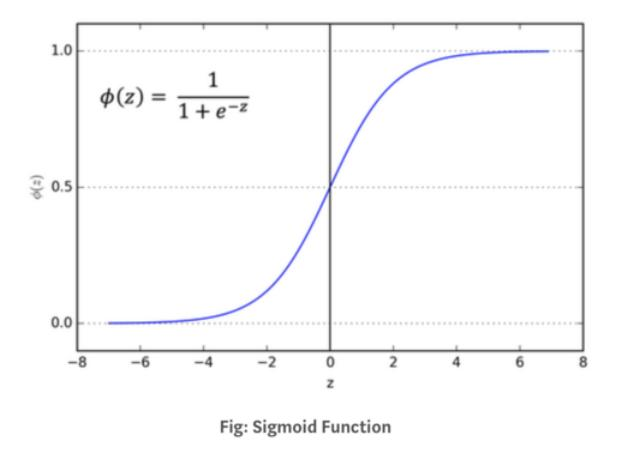
\includegraphics[scale=0.4]{Sigmoid.jpg}
\end{figure}

优点:1.Sigmoid函数的输出映射在(0,1)之间,单调连续,输出范围有限,优化稳定,可以作为输出层。

2.函数连续可导,数学性质好。

缺点:1.由于其软饱和性,导数区间为0——0.25,后向传播时每逆向经过一个节点,梯度值变为原来的四分之一。函数在远离0的两端,导数趋于0,容易产生梯度消失,权重无法更新,导致训练出现问题。

2.其输出并不是以0为中心,会导致我们的模型在优化的过程中收敛速度变慢。在选取参与模型中相关计算的数据时,要尽量使用零中心(Zero-Centered)数据;而且尽量保证计算得到的输出结果时零中心数据。

\begin{Python}{调用Sigmoid函数}
import torch.nn as nn
m = nn.sigmoid()
\end{Python}

\begin{center}
	2.Tanh函数
\end{center}
反曲正切定义为:
$$tanh(x)=\frac{1-e^{-2x}}{1+e^{-2x}}=2\phi(2x)-1$$
$$\frac{\partial tanh(x)}{\partial x}=1-tanh(x)^2$$
\begin{figure}[htbp]
	\centering
	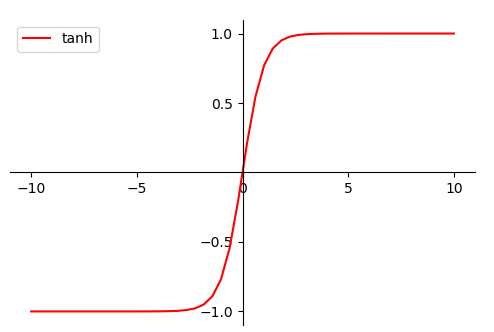
\includegraphics[scale=0.38]{tanh.jpg}
	\caption{tanh函数}
\end{figure}

优点:1.比Sigmoid函数收敛速度更快\\
2.相比Sigmoid函数,其输出以0为中心,解决了偏置问题。

缺点:函数两端的梯度趋于0,没有改变由于饱和性产生的梯度消失,tanh函数的导数取值区间为0-1,仍然不够大。

\begin{Python}{调用Tanh函数}
import torch.nn as nn
m = nn.tanh()
\end{Python}

\begin{center}
	3.ReLU函数
\end{center}
修正线性单元(Rectified Linear Unit,ReLU)函数用来替代传统的激活函数

\begin{figure}[htbp]
	\centering
	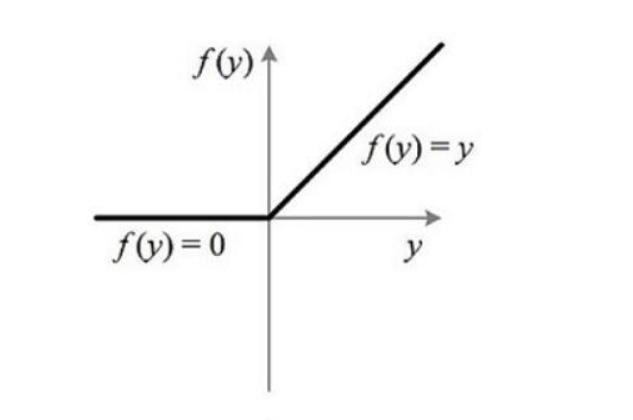
\includegraphics[scale=0.32]{ReLU函数.jpeg}
	\caption{ReLU函数}
\end{figure}


函数定义为:
$$
y = \left\{ \begin{array}{cl}
	0 &  \ (x \le  0) \\
	x &  \ (x > 0)
\end{array} \right.
$$

\begin{Python}{调用ReLU函数}
torch.nn.functional.relu(input,inplace=False)
	
import torch.nn as nn
m = nn.ReLu()
\end{Python}

优点:1.收敛的速度非常快,计算效率很高。\\
2.梯度为0或常数,有效缓解梯度消失的问题。

缺点:1.不是零中心数据,这可能会导致某些神经元不会被激活,并且这些神经元相对应的参数不能被更新。由于模型参数在初始化时使用了全正或全负的值,或者后向传播过程中设置的学习速率太快导致的。

\begin{center}
	4.Softmax函数
\end{center}

hardmax最大的特点就是只选出其中一个最大的值,即非黑即白。Softmax的含义就在于不再唯一的确定某一个最大值,而是为每个输出分类的结果都赋予一个概率值,表示属于每个类别的可能性。下面给出Softmax函数的定义(以第i个节点输出为例):
$$Softmax(z_i)=\frac{e^{z_i}}{\sum_{c=1}^{C}e^{z_c}}$$

其中$z_i$为第i个节点的输出值,C为输出节点的个数,即分类的类别个数。通过Softmax函数就可以将多分类的输出值转换为范围在[0, 1]且和为1的概率分布。

\begin{figure}[htbp]
	\centering
	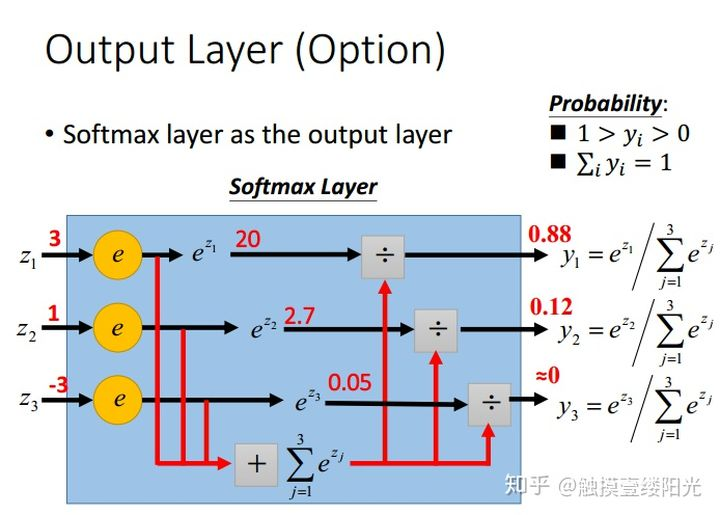
\includegraphics[scale=0.25]{softmax}
\end{figure}

优点:1.指数函数曲线呈现递增趋势,最重要的是斜率逐渐增大,也就是说在x轴上一个很小的变化,可以导致y轴上很大的变化。这种函数曲线能够将输出的数值拉开距离。并且能够避免输出值为负值。

2.使用反向传播求解梯度进而使用梯度下降进行参数更新的过程,而指数函数在求导的时候比较方便。比如:$(e^x)'=e^x$

缺点:1.指数函数的曲线斜率逐渐增大虽然能够将输出值拉开距离,但是也带来了缺点,当$z_i$值非常大的话,计算得到的数值也会变的非常大,数值可能会溢出。当然针对数值溢出有其对应的优化方法,将每一个输出值减去输出值中最大的值。

$D=max(z)$
$$Softmax(z_i)=\frac{e^{z_i-D}}{\sum_{c=1}^{C}e^{z_c-D}}$$

\begin{center}
	5.LReLU
\end{center}
带泄露的ReLU(Leaky ReLU,LReLU)在梯度为0的区域保留一个很小的梯度,以维持参数更新。

$$LReLU(x)= \left\{ \begin{array}{cl}
	x & : \ x > 0 \\
	ax & : \ x \le  0
\end{array} \right.$$
$$\frac{\partial y}{\partial x}=\left\{ \begin{array}{cl}
	1 & : \ x > 0 \\
	a & : \ x \le  0
\end{array} \right.$$
\begin{figure}[htbp]
	\centering
	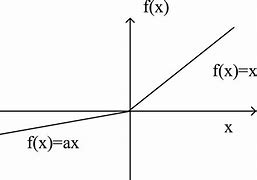
\includegraphics[scale=0.4]{LReLU}
\end{figure}
\begin{center}
	6.PReLU
\end{center}
在ReLU的基础上引入了一个可学习的参数,不同的神经元由不同的参数。
$$LReLU(x)= \left\{ \begin{array}{cl}
	x & : \ x > 0 \\
	a_ix & : \ x \le  0
\end{array} \right.$$
$$\frac{\partial y}{\partial x}=\left\{ \begin{array}{cl}
	1 & : \ x > 0 \\
	a_i & : \ x \le  0
\end{array} \right.$$
\begin{figure}[htbp]
	\centering
	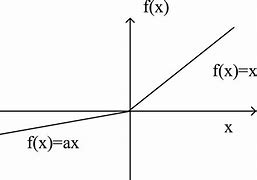
\includegraphics[scale=0.4]{LReLU}
\end{figure}
PReLU神经元中的$\alpha_i$不是一个固定的数,而是每个神经元中可学习的参数,也是一组PReLU神经元共享的参数。当$\alpha=0$时,PReLU看作ReLU,但$\alpha_i$是一个很小的数时,PReLU看作LReLU。
\begin{center}
	7.ELU
\end{center}
指数线性单元(Exponential Linear Unit,ELU)解决了ReLU非零中心化。ELU输出均值接近于0,是一个近似的零中心化的非线性函数。
$$ELU(x)=\left\{ \begin{array}{cl}
	x &  \ x > 0 \\
	\alpha(e^x-1) &  \ x \le  0
\end{array} \right.$$
$$\frac{\partial y}{\partial x}=\left\{ \begin{array}{cl}
	1 & : \ x > 0 \\
	\alpha e^x & : \ x \le  0
\end{array} \right.$$
其中$\alpha$是一个可调整的参数,控制着ELU负值部分的饱和
\begin{figure}[htbp]
	\centering
	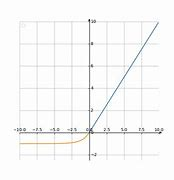
\includegraphics[scale=0.6]{ELU}
\end{figure}
\begin{center}
	8.Maxout
\end{center}
Maxout单元的激活函数是最大值函数max,接收的是神经元的接入,每个Maxout神经元有K个权重向量与偏置。
$$y=max(w_1^Tx+b_1,w_2^Tx+b_2,...,w_K^Tx+b_K)$$
$$\frac{\partial y}{\partial z_k}=\left\{ \begin{array}{cl}
	1 & : \text{$z_k$为最大值} \\
	0 & : \text{其他}
\end{array} \right.$$

只有取最大值的一路保留梯度,其他没有梯度。
\subsection{网络结构}
神经网络:很多神经元连接在一起传递信息来协作完成复杂的功能。

按神经网络的拓扑结构可以分为:前馈神经网络(Feedforward Neural Network),反馈神经网络(Recurrent Neural Network)和图网络(Graph Neural Network)。

\begin{center}
	1.输入层,输出层和隐层
\end{center}
\begin{figure}[htbp]
	\centering
	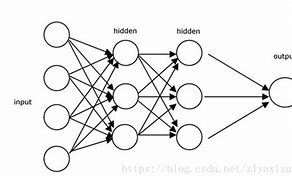
\includegraphics[scale=0.7]{前馈神经网络}
\end{figure}

网络中最左边的一层被称为输入层(Input Layer),其中的神经元被称为输入神经元(Input Neurons)

最右边的一层是输出层(Output Layer),其中的神经元被称为输出神经元(Output Neurons)

网络中处于输入层与输出层之间的层被称为隐层(Hidden Layer)

全连接网络(Fully Connected Network)网络中前一层的所有神经元都与下一层的所有神经元连接。

为了更准确地描述神经网络,引入一些数学符号:对于一个L层的神经网络,第l层有$m^l$个神经元,则l层神经元与前一层的连接权重矩阵为
$$\textbf{W}^l=\begin{bmatrix}
	w_{11}^l & w_{12}^l & \dots & w_{1m^{i-1}}^l \\
	w_{21}^l & w_{22}^l & \dots &  w_{2m^{l-1}}^l\\
	\vdots & \vdots & \ddots & \vdots \\
	w_{m^l1}^l & w_{m^l1}^l & \dots & w_{m^lm^{l-1}}^l
\end{bmatrix}$$
其中$w_{jk}^l$表示第l-1层中的第k个神经元与第l层中的第j个神经元的连接。

l-1层到l层的偏置为:$$\textbf{b}^l = [b_1^l,b_2^l,...,b_{m^l}^l]$$

l层神经元净输入向量为:$$\textbf{z}^l=[z_1^l,z_2^l,...,z_{m^l}^l]$$

l层神经元所用的激活函数为:$$f^i()=[f_i^l(),f_2^i(),...,f_{m^l}^l()]$$

l层神经元激活值向量为:$$\textbf{a}^l=[a_1^l.a_2^l,...,a_{m^l}^l]$$

前馈神经网络的每一层之间的信息传递方式:$$\textbf{a}^l=f^l(\textbf{W}^l\bullet \textbf{a}^{l-1}+\textbf{b}^l)$$

故前馈神经网络的前向传播公式:$$F(x;\textbf{W},\textbf{b})=f^L(\textbf{W}^L\bullet f^{l-1}(\dots\textbf{W}^2\bullet f^1(\textbf{W}^1\bullet x+\textbf{b}^1)+\textbf{b}^2\dots)+\textbf{b}^L)$$

对于神经网路中的第l层的输出$\textbf{a}^L$,可以看作是原始向量x转换到高维空间的特征向量,这个过程称为特征提取,$\textbf{a}^l$也称为第i层的特征向量或特征图(Feature Map)
\begin{center}
	2.万用近似定理及可视化证明
\end{center}
\textbf{万用近似定理(Universal Approximation Theorem)}:表明如果一个前馈神经网络具有线性输出层和至少一层隐藏层,只要给予网络足够数量的神经元,便可以实现以足够高精度来逼近任意一个在实数空间的紧子集上的连续函数。

在此不讨论定理的严格的数学证明。



\subsection{训练与预测}
在训练阶段,需要为神经网络准备好训练数据及对应的标签,通过训练得到一个模型,通过不断地修改网络中所有地权重w和偏置b,使得神经网络地输出尽可能地逼近真实模型的输出。

在预测阶段,在新的测试数据上运行训练好的模型,可以得到分类或者回归的结果。
\begin{center}
	1.损失函数
\end{center}

在神经网络中,衡量网络预测结果和真实值之间的差别的指标称为损失函数(loss fuction)

神经网络的训练就是调整权重w和偏置b使得损失函数值尽量小,在训练过程中,损失函数值逐渐收敛,当其小于设定阈值或设定步数后停止训练,得到一组使得神经网络拟合真实模型的权重和偏置。

神经网络需要解决的是分类问题(输出为有限的离散变量),回归问题(输入变量与输出变量均为连续变量的预测问题)。

(1)分类损失函数
\\\textbf{Logistic损失(Logistic loss)}:
$$loss(\hat{y},y)=\prod_{i=1}^{N}\hat{y}^{y_i}\bullet(1-\hat{y}_i)^{1-y_i}$$
\textbf{负对数似然函数(Negative Log Likelihood loss)}:
$$loss(\hat{y},y)=-\sum_{i=1}^{N}y_i\bullet log\hat{y}_i+(1-y_i)\bullet log(1-\hat{y}_i)$$
\textbf{交叉熵损失(Cross Entropy loss)}:
$$loss(\hat{y},y)=-\sum_{i=1}^{N}\sum_{j=1}^{M}y_{ij}\bullet log\hat{y}_{ij}$$

(2)回归损失函数
\\\textbf{均方误差(MSE:Mean Square Error)函数}也称L2损失:计算的是预测值与真实值之差的平方的期望值,可用于评价数据的变化程度,其得到的值越小,则说明模型的预测值具有越好的精确度。均方函数的计算:
$$MSE=\frac{1}{N}\sum_{i=1}^{N}(y_{true}^i-y_{pred}^i)^2$$
其中$y_{pred}$表示模型的预测值,$y_{true}$表示真实值
\\\textbf{均方根误差(RMSE:Root Mean Square Error)函数}:
计算的是均方误差的算数平方根值,其得到的值越小,则说明模型的预测值具有越好的精确度。均方根函数的计算:
$$RMSE=\sqrt{\frac{1}{N}\sum_{i=1}^{N}(y_{true}^i-y_{pred}^i)^2}$$
\textbf{平均绝对误差(MAE:Mean Absolute Error)函数}也称L1损失:
计算的是绝对误差的平均值,绝对误差即:模型预测值和真实值之间的差的绝对值,能更好地反映预测值误差的实际情况,其得到的值越小,则说明模型的预测值具有越好的精确度。平均绝对误差函数的计算:
$$MAE=\frac{1}{N}\sum_{i=1}^{N}\left| y_{true}^i-y_{pred}^i \right|$$
\textbf{均方对数差损失(Mean Squared Log Error,MSLE)}:
$$MSLE=\frac{1}{N}\sum_{i=1}^{N}(log\hat{y}_i-logy_i)^2$$
\textbf{Huber损失(Huber loss)}:
$$Huber(\hat{y}_i,y_i) = \left\{ \begin{array}{cl}
	\frac{1}{2}(\hat{y}_i-y_i)^2 & |\hat{y}_i-y_i|\le \delta \\
	\delta|\hat{y}_i-y_i|-\frac{1}{2}\delta & \text{其他}
\end{array} \right.$$
$$loss=(\hat{y},y)=\frac{1}{N}\sum_{i=1}^{N}log(cosh(\hat{y}_i-y_i))$$
\textbf{Log-Cosh损失函数(Log-Cosh loss)}:
$$loss(\hat{y},y)=\frac{1}{N}\sum_{i=1}^{N}log(cosh(\hat{y}_i-y_i))$$

L2损失运用最广泛,优化过程更稳定和准确,但对局外点敏感。

L1损失能有效的惩罚局外点,但它导数不连续使得寻找最优解低效。

Huber损失继承L1和L2的优点,但是良好表现依赖与超参数$\delta$。

Log-Cose损失函数拥有Huber损失所有优点,并且在每一点都是二次可导的。

\begin{center}
	2.参数学习
\end{center}

神经网络使用参数学习算法把从数据中学习到的信息保存在参数里面。

对于训练集中的每一个样本计算其损失,那么在整个训练集上的损失为:
$$\hat{y}_i=F(x_i;\textbf{W},\textbf{b})$$
$$loss(\hat{y},\textbf{y})=\frac{1}{N}\sum_{i=1}^{N}L(\hat{y}_i,y_i)$$
其中$\textbf{y}$是标签y对应的one-hot向量表示。有了目标函数和训练样本,可以通过梯度下降算法来学习神经网络的参数,对于神经网络中每一个的权重$\textbf{W}_{jk}^l$和偏置$\textbf{b}_j^l$,其更新方式为:
\begin{equation*}
	\begin{aligned}
	\textbf{W}_{jk}^l&\gets  \textbf{W}_{jk}^l-\eta[\frac{1}{N}\sum_{i=1}^{N}\frac{\partial L(\hat{y}_i,y_i)}{\partial \textbf{W}_{jk}^l}]\\
	&=\textbf{W}_{jk}^l-\eta[\frac{1}{N}\sum_{i=1}^{N}\frac{\partial L(F(x_i;\textbf{W,b})_i,y_i)}{\partial \textbf{W}_{jk}^l}]
	\end{aligned}
\end{equation*}
\begin{equation*}
	\begin{aligned}
		\textbf{b}_{j}^l&\gets  \textbf{b}_{j}^l-\eta[\frac{1}{N}\sum_{i=1}^{N}\frac{\partial L(\hat{y}_i,y_i)}{\partial \textbf{b}_{j}^l}]\\
		&=\textbf{b}_{j}^l-\eta[\frac{1}{N}\sum_{i=1}^{N}\frac{\partial L(F(x_i;\textbf{W,b})_i,y_i)}{\partial \textbf{b}_{j}^l}]
	\end{aligned}
\end{equation*}
其中$\eta$为梯度下降的步长,也称为神经网络的学习率。但是对每个参数逐一求偏导效率很低,计算量大。
\subsection{反向传播算法}
反向传播算法在1970年代由Werbos博士提出,但是直到1986年David Rumelhart,Geoffrey Hinton和Ronald Williams发表的论文中才说明反向传播算法比传统算法更好计算偏导。

前向传播:
$$\textbf{z}^l=\textbf{W}^l\bullet \textbf{a}^{l-1}+\textbf{b}^l$$
$$\textbf{a}^l=f^l(\textbf{z}^l)$$

定义损失关于神经元净输入的偏导数为误差项:$$\delta_j^l=\frac{\partial loss}{\partial z_j^l}$$

对于上式中的权重\textbf{W}和偏置\textbf{b}的偏导数,由链式求导法则可得:
$$\frac{\partial loss}{\partial W_{jk}^l}=\frac{\partial loss}{\partial z_j^l}\frac{\partial z_j^l}{\partial W_{jk}^l}=\delta_j\frac{\partial z_j^l}{\partial W_{jk}^l}$$
$$\frac{\partial loss}{\partial b_j^l}=\frac{\partial loss}{\partial z_j^l}\frac{\partial z_j^l}{\partial b_j^l}=\delta_j\frac{\partial z_j^l}{\partial b_j^l}$$

其中:
$$\frac{\partial z_j^l}{\partial W_{jk}^l}=\frac{\partial (\sum_{k}w_{jk}^la_k^{l-1}+b_j^l)}{\partial W_{jk}^l}=a_k^{l-1}$$
$$\frac{\partial z_j^l}{\partial b_j^l}=\frac{\partial (\sum_{k}w_{jk}^la_k^{l-1}+b_j^l)}{\partial b_j^l}=1$$

而
$$z_k^{l+1}=\sum_jw_{kj}^{l+1}f(z_j^l)+b_k^{l+1}\Rightarrow \frac{\partial z_k^{l+1}}{\partial a_j^l}=w_{kj}^{l+1}\bullet f'(z_j^l)$$
$$\delta_j^l=\frac{\partial loss}{\partial z_j^l}=\sum_{k}\frac{\partial loss}{\partial z_k^{l+1}}\bullet \frac{\partial z_k^{l+1}}{\partial z_j^l}=\sum_k\delta_k^{l+1}\bullet \frac{\partial z_k^{l+1}}{\partial z_j^l}$$
可见第l层的误差项$\delta^l$需要通过第l+1层的误差项$\delta^{l+1}$,这与神经网络预测时信息的传递方向(前向传播)正好相反,所以称为方向传播。

误差项最后推导需要从神经网络的最后一层(即输出层)开始往前推,故输出层的误差项$\delta_j^L$的计算方法不同,其梯度来自最后的损失函数:
$$\delta_j^L= \frac{\partial loss}{\partial z_j^L}=\frac{\partial loss}{\partial a_j^L}\bullet \frac{\partial a_j^L}{\partial z_j^L}=\frac{\partial loss(\hat{y}_i,y_i)}{\partial a_j^L}\bullet f'(z_j^L)$$

重写反向传播算法的方程:
$$\delta_j^L=\frac{\partial loss(\hat{y}_i,y_i)}{\partial a_j^L}\bullet f'(z_j^L)=\nabla_aL\bigodot f'(z^L)$$
$$\delta_j^l=\sum_{k}\delta_k^{l+1}\bullet \frac{\partial z_k^{l+1}}{\partial z_j^l}w_{kj}^{l+1}f'(z_j^l)=((\textbf{W}^{l+1})^T\delta^{l+1})\bigodot f'(z^l)$$
$$\frac{\partial loss}{\partial w_{jk}^l}=a_k^{l-1}\delta_j^l\Rightarrow \frac{\partial L}{\partial \textbf{W}^l}=\delta^l(\textbf{a}^{l-1})^T$$
$$\frac{\partial loss}{\partial b_j^l}=\delta_j^l\Rightarrow \frac{\partial L}{\partial \textbf{b}^l}=\delta^l$$

根据反向传播的公式,给出反向传播算法的具体步骤:

(1)前向传播:输入x,计算每一层的净输入:$\textbf{z}^l=\textbf{W}^l\bullet \textbf{a}^{l-1}+\textbf{b}^l$与激活值:$\textbf{a}^l=f^l(\textbf{z}^l)$

(2)计算误差值:计算L层误差项:$\delta_j^L=\nabla_aL\bigodot f'(z^L)$,反向传播计算每一层的误差项:$\delta_j^l=((\textbf{W}^{l+1})^T\delta^{l+1})\bigodot f'(z^l)$

(3)计算每一层权重的偏导:$\frac{\partial L}{\partial \textbf{W}^l}=\delta^l(\textbf{a}^{l-1})^T$和偏置的偏导$\frac{\partial L}{\partial \textbf{b}^l}=\delta^l$,并更新参数。

反向传播算法基于链式法则,合并了许多重复运算,只需要进行一次前向传播与一次反向传播,就可以计算所有参数的梯度,极大地提升了梯度计算的速度。

\subsection{代码实现}
\begin{Python}{前馈神经网络}
	#相关包的导入
	import torch
	import torch.nn as nn
	import torchvision.datasets as dsets
	import torchvision.transforms as transforms
	from torch.autograd import Variable
	import torch.utils.data as Data
	import matplotlib.pyplot as plt
	
	#定义输入,输出和权重参数
	input_size = 784
	hidden_size = 500
	num_classes = 10
	num_epochs = 5
	batch_size = 100
	learning_rate = 0.001
	train_dataset = dsets.MNIST(root='./data', train=True, transform=transforms.ToTensor(), download=True)
	test_dataset = dsets.MNIST(root='./data', train=False, transform=transforms.ToTensor())
	
	train_loader = torch.utils.data.DataLoader(dataset=train_dataset, batch_size=batch_size, shuffle=True)
	test_loader = torch.utils.data.DataLoader(dataset=test_dataset, batch_size=batch_size, shuffle = False)
	
	#_device = torch.device('cuda:0')
	
	#定义好神经网络
	class Net(nn.Module):
	def __init__(self, input_size, hidden_size, num_classes):
	super(Net, self).__init__()
	self.fc1 = nn.Linear(input_size, hidden_size)
	self.relu = nn.ReLU()
	self.fc2 = nn.Linear(hidden_size, num_classes)
	def forward(self, x):
	out = self.fc1(x)
	out = self.relu(out)
	out = self.fc2(out)
	return out
	
	# def dict_all_to_device(tensor_dict, device):
	#     for k in tensor_dict:
	#         if isinstance(tensor_dict[k], torch.Tensor):
	#             tensor_dict[k] = tensor_dict[k].to(device)
	
	net = Net(input_size, hidden_size, num_classes)
	criterion = nn.CrossEntropyLoss()
	optimizer = torch.optim.Adam(net.parameters(), lr=learning_rate)
	
	#对模型进行正式训练并对参数进行优化
	for epoch in range(num_epochs):
	for i, (images, labels) in enumerate(train_loader):
	# dict_all_to_device(images, _device)
	# dict_all_to_device(labels, _device)
	images = Variable(images.view(-1, 28*28))
	labels = Variable(labels)
	optimizer.zero_grad()
	#把图片信息传给outputs
	outputs = net(images)
	#计算损失函数
	loss = criterion(outputs, labels)
	loss.backward()
	#更新参数
	optimizer.step()
	if (i+1) % 100 == 0:
	print('Epoch [%d/%d], step [%d/%d], Loss: %.4f'
	%(epoch + 1, num_epochs, i + 1, len(train_dataset)//batch_size, loss))
	
	correct = 0
	total = 0
	for images, labels in test_loader:
	images = Variable(images.view(-1, 28*28))
	outputs = net(images)
	_, predicted = torch.max(outputs.data, 1)
	total += labels.size(0)
	correct += (predicted == labels).sum()
	#输出精度
	print('Accuracy of the network on the 10000 test images: %d %%' % (100 * correct / total))
	
	#Output:Epoch [5/5], step [400/600], Loss: 0.0177
	#		Epoch [5/5], step [500/600], Loss: 0.0049
	#		Epoch [5/5], step [600/600], Loss: 0.0071
	#		Accuracy of the network on the 10000 test images: 97 %
\end{Python}
\section{提升神经网络训练的技巧}
\subsection{参数更新方法}
\begin{center}
	1.批量梯度下降(Batch Gradient Descent,BGD)
\end{center}

运用线性模型来进行说明。给定包含m个样本的数据集,每个样本由n个属性描述。试图用$x_{ij}$表示$y_i$,$x_{ij}$是第i个样本在第j个属性上的取值。
$$
\begin{pmatrix}
	x_{11} &x_{12}  &x_{13}  & \dots &x_{1n}  \\
	x_{21} &x_{22}  &x_{23}  & \dots &x_{2n} \\
	x_{31} &x_{32}  &x_{33}  & \dots &x_{3n}  \\
	\vdots&\vdots  &\vdots  &  &\vdots  \\
	x_{m1} &x_{m2}  &x_{m3}  & \dots &x_{mn}
\end{pmatrix} _{m\times n}
$$
我们试图用线性组合的方式$x_ij$表示$y_i$

故第一个样本数据集,预测值为:
$$h_1(\theta) =\sum_{j=1}^{n}\theta_{1j}x_{1j}=\theta_{11}x_{11}+\theta_{12}x_{12}+\dots+\theta_{1n}x_{1n}$$

第一个样本的损失为:
$$J_1=\frac{1}{2}(\sum_{j=1}^{n}\theta_{1j}x_{1j}-y_1)^2$$

总损失平均为:
$$J=\frac{1}{2}\frac{1}{m}\sum_{i=1}^{m}(\sum_{j=1}^{n}\theta_{ij}x_{ij}-y_i)^2$$

我们目的是使损失函数尽可能的小,线性组合中的$\theta_j$看成m个样本各自线性组合算出的$\theta_{ij}$取和的平均。

对第一个样本求取$\theta_{1j}$的偏导:
$$\frac{\partial J_1}{\partial \theta_j}=(\sum_{j=1}^{n}\theta_{1j}x_{1j}-y_1)\sum_{j=1}^{n}x_{1j}\}$$

对m个样本总损失求取$\theta_j$的偏导数:
$$\frac{\partial J}{\partial \theta_j}=\frac{1}{m}\sum_{i=1}^{m}\{(\sum_{j=1}^{n}\theta_{ij}x_{ij}-y_i)\sum_{j=1}^{n}x_{ij}\}$$

对m个样本中相对应的第j个参数进行更新:
$$\theta_j \Leftarrow \theta_j - \eta \frac{1}{m} \sum_{i=1}^{m}\{(\sum_{j=1}^{n}\theta_{ij}x_{ij}-y_i)\sum_{j=1}^{n}x_{ij}\}$$

优点:
(1)一次迭代是对所有样本进行计算,此时利用矩阵进行操作,实现了并行。
(2)由全数据集确定的方向能够更好地代表样本总体,从而更准确地朝向极值所在的方向。当目标函数为凸函数时,BGD一定能够得到全局最优。

缺点:
当样本数目 m 很大时,每迭代一步都需要对所有样本计算,训练过程会很慢。

\begin{center}
	2.随机梯度优化算法SGD(Stochastc Gradient Descent)
\end{center}
每次从训练集中随机采样第i个样本第j个属性计算loss和梯度,然后更新参数。
$$\theta \Leftarrow \theta-\eta \bullet \nabla F(x^{ij},y^{ij};\theta)$$
每次从训练集中随机采样m个样本对第j个属性组成一个小批量(Mini-Batch)来计算loss和梯度:
$$\theta \Leftarrow \theta-\eta \bullet \nabla \sum_{i}^{i+m}F(x^{i,j},y^{i,j};\theta)$$

优点:训练速度快,对于很大的数据集,也能够以很快的速度收敛。但是选择合适的学习速率比较困难,合适的学习率对算法收敛很重要。

缺点:1.对于非凸函数,SGD容易陷入局部极小值处或者鞍点处,使得SGD在鞍点处震荡,难以逃出这一区域。
2.SGD对所有参数更新时使用相同的学习率,但会有对不同的特征进行不同程度的更新的需求。

torch.optim.SGD(params, lr=,momentum=0,dampening=0,\\weight\_dacay=0,nesterov=False)

由于是抽取,得到的梯度有误差,故学习速率需要逐渐减小。因为误差,每次迭代的梯度受抽样的影响比较大,梯度含有较大的噪声,不能很好的反映真实梯度。
\begin{Python}{SGD算法}
optimizer = torch,optim.SGD(model.parameters(), lr=0.1, momentum=0.9)
optimizer.zero_grad()
loss_fn(model(input, target).backward()
optimizer.step()
\end{Python}

\begin{center}
3.Momentum
\end{center}
为克服SGD陷入局部极小值,引入动量(momentum)。在梯度上加入这一项,可以使得梯度在方向不变的维度上速度变快,方向有所改变的维度上的更新速度变慢,有助于加快收敛并减少震荡。

保留了上一步的梯度:
$$\nu_t=\mu\nu_{t-1}+\eta\nabla _\theta F(\theta)$$
$$\theta \Leftarrow \theta - \nu_t$$
$\mu$为动量因子,一般取值为0.9

\begin{center}
	4.Nesterov加速梯度NAG(Nesterov Accelerated Gradient)
\end{center}
不仅考虑历史梯度信息,并把历史梯度信息运用于下一次的迭代中。
$$\nu_t=\mu\nu_{t-1}+\eta\nabla _\theta F(\theta-\mu\nu_{t-1})$$
$$\theta \Leftarrow \theta - \nu_t$$
更新梯度时顺应loss的梯度来调整速度,对SGD进行加速。

\begin{center}
	5.Adagrad
\end{center}
一种自适应算法,可以根据参数更新的频率来调整它们更新的幅度,对低频的参数做较大的更新,对高频的参数做较小的更新。

引入一个梯度的累计项$G_{t,ii}=\sum_{i=1}^{t}g_{t,i}^2$,其中$g_{t,i}$表示t时刻参数$\theta_i$的梯度,$G_{t,ii}$为一个对角矩阵,其梯度更新公式:
$$\theta_{t+1}\leftarrow \theta_t- \frac{\eta}{\sqrt{G_t+\xi}}\bigodot g_t$$
式中$\xi$是小正实数,$\eta$取0.01.

对于式中可以经常更新的参数$\theta_i$,其$G_{t,ii}$会累积较快,以抵制学习率。对于式中不经常更新的参数$\theta_j$,其$G_{t,jj}$的值较小,以获得较大学习率。

但分母会不断积累,导致学习率快速下降,最后变得很小,导致参数更新小而难以趋于最优解。
\begin{center}
	6.Adadelta
\end{center}
Adadelta是对Adagrad的扩展,最初方案依然是对学习率进行自适应约束,但是进行了计算上的简化。 Adagrad会累加之前所有的梯度平方,而Adadelta只累加固定大小的项,并且也不直接存储这些项,仅仅是近似计算对应的平均值。即:

$$G_t=\gamma g_{t-1}^2+(1-\gamma)g_t^2$$

对上式两边重写开根,用均方根(Root Mean Squared,RMS)表示:
$$RMS[g]_t=\sqrt{G_t+\varepsilon}=\sqrt{\gamma g_{t-1}^2+(1-\gamma)g_t^2+\varepsilon}$$

故Adagrad能重写为
$$\theta_{t+1}\leftarrow \theta_t- \frac{\eta}{RMS[g]_t}\bigodot g_t$$

但是发现单位不一致,对梯度的变化量也构造了均方根,
$$RMS[\Delta \theta_i]=\sqrt{E[\Delta \theta ^2]_t+\varepsilon}$$

故整个梯度更新写作:
$$\Delta \theta_t=-\frac{RMS[\Delta \theta]_{t-1}}{RMS[g]_t}\bigodot g_i$$
$$\theta_{t+1}=\theta_t + \Delta \theta_t$$
\begin{center}
	7.RMSprop
\end{center}
用滑动平均的方法解决Adagrad学习率急剧下降的问题,使用一个滑动窗口限制G,此时的G为滑动窗口求得的平均值,

批量梯度下降法是最原始的形式,它是指在每一次迭代时使用所有样本来进行梯度的更新。
$$G_t=\gamma G_{t-1}^2+(1-\gamma)g_t^2$$
$$\theta_{t+1}\leftarrow \theta_t- \frac{\eta}{\sqrt{{G_t+\varepsilon}}}\bigodot g_t$$
其中平衡因子$\gamma$为0.9,学习率$\eta$为0.001
\begin{center}
	8.自适应矩估计Adam(Adaptive Moment Estimation)
\end{center}
结合了基于动量的优化方法与基于自适应学习率的优化方法,它保存了过去梯度的指数衰减平均值(梯度的一阶矩),将其作为动量与过去梯度的平方的指数衰减平均值(梯度的二阶矩)来构造学习率自适应因子。
$$m_t=\gamma_1m_{t-1} + (1-\gamma_1)g_1$$
$$v_t=\gamma_2v_{t-1} + (1-\gamma_2)g_t^2$$
并对梯度的一阶矩和二阶矩做了偏差矫正:
$$\hat{m}_t = \frac{m_t}{1-\gamma_1^t}$$
$$\hat{v}_t = \frac{v_t}{1-\gamma_2^t}$$
其梯度更新表示式为:
$$\theta_{t+1}=\theta_t - \frac{\eta}{\sqrt{\hat{v_t}}+\xi}\bigodot \hat{m}$$
超参数的建议值为$\gamma_1=0.9,\gamma_2=0.999,\xi=1\times 10^{-8}$
\begin{center}
	9.AdaMax
\end{center}
对Adam进行改进,使用梯度的无穷矩来构造学习率自适应因子,动量依然为梯度的一阶矩。
$$m_t=\gamma_1m_{t-1} + (1-\gamma_1)g_1$$
$$v_t=\gamma_2^{\infty}v_{t-1} + (1-\gamma_2^{\infty})|g_t|^{\infty}=max(\gamma_2\bullet v_{t-1},|g_t|)$$
此时无穷矩不是有偏的,无须校正,其梯度更新如下:
$$\theta_{t+1}=\theta_t - \frac{\eta}{\hat{v_t}+\xi}\bigodot \hat{m}$$
超参数的建议值为$\gamma_1=0.9,\gamma_2=0.999,\eta = 0.002$
\begin{center}
	10.Nadam
\end{center}
在Adan的基础上结合NAG,Nadam修改了梯度的一阶矩,梯度的二阶矩不变。
$$\theta_{t+1}=\theta_t - \frac{\eta}{\sqrt{\hat{v_t}}+\xi}[\gamma_1\hat{m}+\frac{(1-\gamma_1)g_t}{1-\gamma_1^t}]$$
\subsection{数据预处理}
一般对数据进行归一化(normalization)会对深度学习算法的效率有很大提高。
三种常用的数据预处理方法:

\textbf{1.0均值}:所有样本减去总体数据的平均值,适用于各维度分布相同的数据$x-E(x)$

\textbf{2.缩放}:将不同维度差异较大的数据缩放到统一的尺寸以利于模型处理
$$\frac{x}{a}\in [0,1]^R \text{或} \frac{x}{a}\in [-1,1]^R$$

\textbf{3.归一化}:各维度数据减去各维度的均值后除以各维度的标准差$$\frac{x-E(x)}{\sigma(x)}$$
\subsection{参数的初始化}
神经网络与深度学习的优化是非凸的,权重的初始值会导致不同的结果和收敛速度。
\begin{center}
	1.全零初始化
\end{center}
全零初始化即将所有变化初值设为0,在神经网络中常用于对偏置值b的初始化。而对于权重不使用全零初始化。
\begin{center}
	2.随机初始化
\end{center}
随机值初始化即在0附近取随机值初始化权重w,随机值初始化打破这种神经元之间的对称型,使得神经网络可学习。但由于权重所取的太小很难与神经元的数量关系平衡,使得网络训练收敛慢甚至失败。

放大权重使得每层的梯度处于相似的区间,不过此时净输入值过宽,使得激活值基本处于二值状态,神经网络的能力退化。
\begin{center}
	3.Xavier初始化(Glorot初始化)
\end{center}
目的是使得梯度,净输入值和激活值在所有层上相似,即保持所用层的方差相似。常与sigmoid激活函数和tanh激活函数搭配使用。

Xavier初始化根据输入和输出神经元的数量自动决定初始化的范围,定义参数所在层的输入维度为$fan_{in}$,输出维度为$fan_{out}$,则权重\textbf{W}可从正太分布中进行采样:
$$\textbf{W}\sim N(0,\sqrt{\frac{2}{fan_{in}+fan_{out}}})$$
权重\textbf{W}可从均匀分布U中进行采样:
$$\textbf{W}\sim N(-\sqrt{\frac{6}{fan_{in}+fan_{out}}},\sqrt{\frac{6}{fan_{in}+fan_{out}}})$$
\begin{center}
	4.He初始化(MSRA初始化)
\end{center}
针对神经网络使用ReLU函数是的权重初始化方案,ReLU激活函数让一半的净输入值(负值)变为零,可认为移除了大约一般的方差,所以需要加倍权重的方差以补偿这一点。则权重\textbf{W}可在正太分布中采样:
$$\textbf{W}\sim M(0,\sqrt{\frac{4}{fan_{in}+fan_{out}}})$$
$$\textbf{W}\sim M(0,\sqrt{\frac{2}{fan_{in}}})$$
权重\textbf{W}可从均匀分布U中进行采样:
$$\textbf{W}\sim N(-\sqrt{\frac{6}{fan_{in}}},\sqrt{\frac{6}{fan_{in}}})$$
\subsection{正则化}
正则化用于解决有些模型因强大的表征能力而产生测试数据过拟合等现象,通过避免训练完美拟合数据样本的模型来加强算法的泛化能力。
为了防止过拟合有以下的解决的方法:增加训练样本数量,使用数据加强,权重衰减(L1/L2正则化),Dropout和提前停止(Early stopping)

\begin{center}
	1.数据加强
\end{center}
数据加强通过向训练数据添加转换或扰动来人工增加训练数据集。考虑到增加噪声的多样性,可以添加多种噪声以获取更多的数据。在计算机视频应用中,数据增强常用的手段有水平或垂直翻转图像,裁剪,色彩变换,缩放和旋转
\begin{center}
	2.权重衰减
\end{center}

L2指二范数,常写成平方和的形式,L2正则化中,添加正则化项以减少参数平方的总和,L2正则化公式:
$$L=loss(y,\hat{y})+\frac{\lambda}{2n}\sum w^2$$
其中n为训练样本的总数,$\lambda$为正则化系数,$\lambda$越小正则化作用越小,模型主要优化原本的损失函数;$\lambda$越大正则化作用越明显,权重w趋于0。

求导后:$$\frac{\partial L}{\partial w}=\frac{\partial loss(y,\hat{y})}{\partial w}+\frac{\lambda}{n}w$$
代入w的更新公式:
$$w \Leftarrow (1-\eta \frac{\lambda}{n})w-\eta \frac{\partial L}{\partial w}$$

L1指一范数,常写成绝对值和的形式,L1正则化中,向目标函数添加正则化项以减少参数绝对值总和,L1正则化公式:
$$L=loss(y,\hat{y})+\frac{\lambda}{n}\sum |w|$$
其中n为训练样本的总数,$\lambda$为正则化系数,$\lambda$越小正则化作用越小,模型主要优化原本的损失函数;$\lambda$越大正则化作用越明显,权重w趋于0。

求导后:$$\frac{\partial L}{\partial w}=\frac{\partial loss(y,\hat{y})}{\partial w}+\frac{\lambda}{n}sign(w)$$
代入w的更新公式:
$$w \Leftarrow (1-\eta \frac{\lambda}{n}sign(w))w-\eta \frac{\partial L}{\partial w}$$
\begin{center}
	3.Dropout(Drop Connect)
\end{center}
指暂时丢弃一部分神经元及其连接。可通过阻止某些特征的协同作用来缓解,每次训练的时候,每个神经元有p的概率被移除,让一个神经元的出现依赖于另一个神经元。每个神经元被关闭的概率是相同的。我们通过调整概率p为较小的值来防止过拟合现象。

\begin{figure}[htbp]
	\centering
	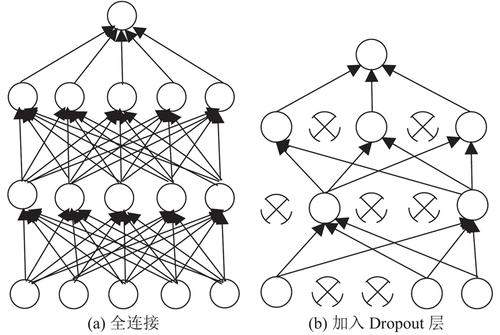
\includegraphics[scale=2.7]{Dropout.jpg}
\end{figure}
\begin{center}
	4.提前停止
\end{center}
提前停止(early stop)可以限制模型最小化代价函数所需的训练迭代次数,提前停止通常用于防止训练中过拟合的模型泛化性能差。
\begin{figure}[htbp]
	\centering
	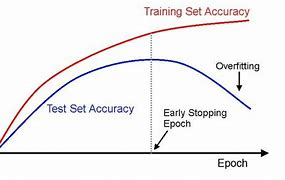
\includegraphics[scale=0.5]{early stop}
\end{figure}
\section{深度学习框架}
\subsection{深度学习框架的作用}
降低了深度学习入门的门槛,通过提供一系列深度学习的组件,就可以避免重复发面轮子,而专注于技术研究和产品创新。

易用性:可使深度学习模型的设计如同编写伪代码一样容易,只需要关注高层结构,不必担心底层问题。

高效性:能够使用集群分布式进行计算或者使用多GPU进行计算,因此使用具有分布式性能的深度学习框架可以使模型训练更高效。
\subsection{常见深度学习框架}
飞桨:百度提供的国内首个开源深度学习框架,极大地提升了框架对模型地表达能力。

TensorFlow:Google推出的机器学习开源工具,主要应用于机器学习和深度神经网络研究。

Caffe:由神经网络中的表达式,速度及模块化产生的深度学习框架。在Linux上,C++可以通过命令行来操作接口,运算上支持CPU和GPU直接无缝切换。

Keras:基于Python开发的极其精简并高度模块化的神经网络库,支持CPU和GPU运算。

\section{手写数字识别代码实现}
\begin{Python}{代码实现}
import torch
import torch.nn as nn
import torch.utils.data as Data
import torchvision
import matplotlib.pyplot as plt
import os
import cv2

torch.manual_seed(1)  # 使用随机化种子使神经网络的初始化每次都相同

# 超参数
EPOCH = 1  # 训练整批数据的次数
BATCH_SIZE = 50
LR = 0.001  # 学习率
DOWNLOAD_MNIST = True  # 表示还没有下载数据集,如果数据集下载好了就写False

# 下载mnist手写数据集
train_data = torchvision.datasets.MNIST(
root='./data/',  # 保存或提取的位置  会放在当前文件夹中
train=True,  # true说明是用于训练的数据,false说明是用于测试的数据
transform=torchvision.transforms.ToTensor(),  # 转换PIL.Image or numpy.ndarray

download=DOWNLOAD_MNIST,  # 已经下载了就不需要下载了
)

test_data = torchvision.datasets.MNIST(
root='./data/',
train=False  # 表明是测试集
)

# 批训练 50个samples, 1  channel,28x28 (50,1,28,28)
# Torch中的DataLoader是用来包装数据的工具,它能帮我们有效迭代数据,这样就可以进行批训练
train_loader = Data.DataLoader(
dataset=train_data,
batch_size=BATCH_SIZE,
shuffle=True  # 是否打乱数据,一般都打乱
)

# 进行测试
# 为节约时间,测试时只测试前2000个
#
test_x = torch.unsqueeze(test_data.train_data, dim=1).type(torch.FloatTensor)[:2000] / 255
# torch.unsqueeze(a) 是用来对数据维度进行扩充,这样shape就从(2000,28,28)->(2000,1,28,28)
# 图像的pixel本来是0到255之间,除以255对图像进行归一化使取值范围在(0,1)
test_y = test_data.test_labels[:2000]


# 用class类来建立CNN模型
# CNN流程:卷积(Conv2d)-> 激励函数(ReLU)->池化(MaxPooling)->
#        卷积(Conv2d)-> 激励函数(ReLU)->池化(MaxPooling)->
#        展平多维的卷积成的特征图->接入全连接层(Linear)->输出

class CNN(nn.Module):  # 我们建立的CNN继承nn.Module这个模块
def __init__(self):
super(CNN, self).__init__()
# 建立第一个卷积(Conv2d)-> 激励函数(ReLU)->池化(MaxPooling)
self.conv1 = nn.Sequential(
# 第一个卷积con2d
nn.Conv2d(  # 输入图像大小(1,28,28)
in_channels=1,  # 输入图片的高度,因为minist数据集是灰度图像只有一个通道
out_channels=16,  # n_filters 卷积核的高度
kernel_size=5,  # filter size 卷积核的大小 也就是长x宽=5x5
stride=1,  # 步长
padding=2,  # 想要con2d输出的图片长宽不变,就进行补零操作 padding = (kernel_size-1)/2
),  # 输出图像大小(16,28,28)
# 激活函数
nn.ReLU(),
# 池化,下采样
nn.MaxPool2d(kernel_size=2),  # 在2x2空间下采样
# 输出图像大小(16,14,14)
)
# 建立第二个卷积(Conv2d)-> 激励函数(ReLU)->池化(MaxPooling)
self.conv2 = nn.Sequential(
# 输入图像大小(16,14,14)
nn.Conv2d(  # 也可以直接简化写成nn.Conv2d(16,32,5,1,2)
in_channels=16,
out_channels=32,
kernel_size=5,
stride=1,
padding=2
),
# 输出图像大小 (32,14,14)
nn.ReLU(),
nn.MaxPool2d(2),
# 输出图像大小(32,7,7)
)
# 建立全卷积连接层
self.out = nn.Linear(32 * 7 * 7, 10)  # 输出是10个类

# 下面定义x的传播路线
def forward(self, x):
x = self.conv1(x)  # x先通过conv1
x = self.conv2(x)  # 再通过conv2
# 把每一个批次的每一个输入都拉成一个维度,即(batch_size,32*7*7)
# 因为pytorch里特征的形式是[bs,channel,h,w],所以x.size(0)就是batchsize
x = x.view(x.size(0), -1)  # view就是把x弄成batchsize行个tensor
output = self.out(x)
return output


cnn = CNN()
#print(cnn)

# 训练
# 把x和y 都放入Variable中,然后放入cnn中计算output,最后再计算误差

# 优化器选择Adam
optimizer = torch.optim.Adam(cnn.parameters(), lr=LR)
# 损失函数
loss_func = nn.CrossEntropyLoss()  # 目标标签是one-hotted

# 开始训练
# for epoch in range(EPOCH):
#     for step, (b_x, b_y) in enumerate(train_loader):  # 分配batch data
#         output = cnn(b_x)  # 先将数据放到cnn中计算output
#         loss = loss_func(output, b_y)  # 输出和真实标签的loss,二者位置不可颠倒
#         optimizer.zero_grad()  # 清除之前学到的梯度的参数
#         loss.backward()  # 反向传播,计算梯度
#         optimizer.step()  # 应用梯度
#
#         if step % 50 == 0:
#             test_output = cnn(test_x)
#             pred_y = torch.max(test_output, 1)[1].data.numpy()
#             accuracy = float((pred_y == test_y.data.numpy()).astype(int).sum()) / float(test_y.size(0))
#             print('Epoch: ', epoch, '| train loss: %.4f' % loss.data.numpy(), '| test accuracy: %.2f' % accuracy)
#
# torch.save(cnn.state_dict(), 'cnn2.pkl')#保存模型


# 加载模型,调用时需将前面训练及保存模型的代码注释掉,否则会再训练一遍
cnn.load_state_dict(torch.load('cnn2.pkl'))
cnn.eval()
# print 10 predictions from test data
inputs = test_x[:100]  # 测试100个数据
test_output = cnn(inputs)
pred_y = torch.max(test_output, 1)[1].data.numpy()
print(pred_y, 'prediction number')  # 打印识别后的数字
# print(test_y[:10].numpy(), 'real number')

img = torchvision.utils.make_grid(inputs)
img = img.numpy().transpose(1, 2, 0)

# 下面三行为改变图片的亮度
# std = [0.5, 0.5, 0.5]
# mean = [0.5, 0.5, 0.5]
# img = img * std + mean
cv2.imshow('win', img)  # opencv显示需要识别的数据图片
key_pressed = cv2.waitKey(0)
\end{Python}
\section{强化学习}
深度学习的另一个最大的成就是其在 强化学习(reinforcement learning)领域的扩展。在强化学习中,一个自主的智能体必须在没有人类操作者指导的情况下,通过试错来学习执行任务。

\section{Others}

最简单的前馈网络,主要用于模式分类,基于模式分类的学习控制和多模态控制中。感知器网络可分为单层感知器网络和多层感知器网络。

\begin{center}
	2.BP网络
\end{center}

连接权调整采用反向传播(Back Propagation)学习算法的前馈网络。与感知器不同之处在于,BP网络的神经元变换函数采用了Sigmoid函数,导致输出量是0-1之间的连续值,可实现从输入到输出的任意的非线性映射。

\begin{center}
	3.RBF网络
\end{center}

隐含层神经元由RBF神经元(神经元的变化函数为Radial Basis Function 径向基函数)组成的前馈网络。

典型的RBF网络由三层组成:一个输入层,一个或多个由RBF神经元组成的RBF层(隐含层),一个由线性神经元组成的输出层。

多层感知机,每个圆圈是一个神经元,每条线表示神经元之间的连接。层与层之间的神经元有连接,层内之间的神经元没有连接。
\begin{figure}[htbp]
	\centering
	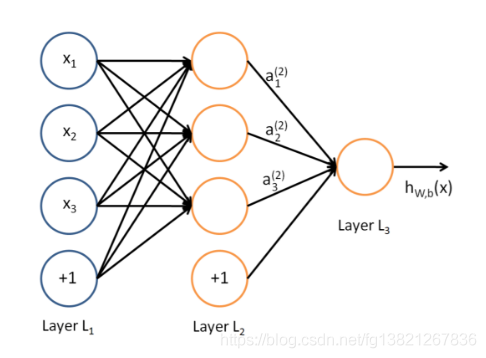
\includegraphics[scale=0.4]{多层感知机.png}
	\caption{简单的多层感知机}
\end{figure}

最左边的层为输入层:负责接收输入数据。
最右边的层为输出层:从这层获得神经网络输出数据。
输入层和输出层之间的层叫做隐藏层。

感知器以一个实数值向量作为输入,计算输入的线性组合,如果结果大于某个阈值就输出1,否则输出-1。$x_1,x_2,x_3$是输入单元,每个单元代表一个特征。每个输入有一个权值$w_i$,还有一个偏置项$w_0$。每一个$w_i$是一个实数常量,或叫做权值。

感知机通过使用激励函数(Activation Function)处理解释变量和模型参数的线性组合对样本分类。

\begin{equation*}
	O(x_1,...x_n) = \left\{ \begin{array}{cl}
		1 & if \ w_0+w_1x_1+w_2x_2+...+w_nx_n >0 \\
		-1 & otherwise
	\end{array} \right.
\end{equation*}


前馈神经网络由一个输入层,一个或多个隐藏层和一个输出层组成。前馈神经网络结构包括:输入层的单元数,隐藏层数,每个隐藏层的单元数和输出层的单元数。

神经网络可以用于分类(预测给定元组的类标号)和数值预测(预测连续值输出)。隐含层的神经元数目多少决定了多层前馈神经网络的可区分性能,同时计算的复杂性由隐含层的神经元多少决定。

损失函数(Loss Funcation)用来估量模型的预测值与真实值的不一致程度,是一个非实数值函数。损失函数越小,模型的鲁棒性就越好。损失函数是经验风险函数的核心部分,也是结构风险函数重要组成部分。

常见的损失函数由:Log对数损失函数,平方损失函数,指数损失函数(Adaboost),Hinge损失函数,最小二乘损失函数,交叉熵损失函数,KL散度损失函数,负的log likelihood损失函数。



\subsection{数据集}

torchvision.datasets包含的数据集:MNIST,COCO,LSUN Classfication,\\ ImageFolder,Imagenet-12,CIFAR10 anf CIFAR100,STL10,SVHN,Photo Tour。

torchvision.models模块的子模块包含以下预训练的模型结构:AlexNet,\\ VGGNet,ResNet,SqueezeNet,DenseNet。

可以通过构造函数来构造具有随机权重的模型:
\begin{Python}{模型的调用}
	import torchvision.models as models
	resnet18 = models.resnet18()
	alexnet = models.alexnet()
	squeezenet = models.squeezenet1_0()
	densent = models.densenet161()
\end{Python}

Torch.nn包里包含Module神经网络模型,Function函数,通过Optim实现各种优化算法。

Module是神经网络的基本组成部分,作为一个抽象类,可以通过定义成员函数实现不同的神经网络结构。

Functional包括Convolution函数,Pooling函数,非线性激活函数,Normalization函数,线性函数,Dropout函数,Distance函数,Loss函数。

Optim包含各种优化算法:Momentum算法,NesterovMomentum算法,AdaGrad算法,RMSProp算法,Adam(Adaptive Moment Estimation)算法

\subsection{卷积层}

卷积是一种局部操作,通过一定大小的卷积核作用于局部图像区域,从而得到图像的局部信息。

一维卷积层:
class torch.nn.Conv1d(in\_channels,out\_channels,kernel\_size,stride=1,padding=0,dilation=1,groups=1,bias=True)

池化层:
class torch.nn.MaxPool1d(kernel\_size,stride=None,padding=0,dilation=1,return\_indices=False,ceil\_mode=False)

我们用nn包来定义我们的神经网络,创建一个经常性网络,只需多次使用相同的线性图层,无需考虑分享权重。

\begin{Python}{小型ConvNet}
	import torch
	from torch.autograd import Variable
	import torch.nn as nn
	import torch.nn.functional as F
	
	class MNISTConvNet(nn.Module):
	def __init__(self):
	super(MNISTConvNet, self).__init__()
	self.conv1 = nn.Conv2d(1, 10, 5)
	self.pool1 = nn.MaxPool2d(2, 2)
	self.conv2 = nn.Conv2d(10, 20, 5)
	self.pool2 = nn.MaxPool2d(2, 2)
	self.fc1 = nn.Linear(320, 50)
	self.fc2 = nn.Linear(50, 10)
	def forward(self, input):
	x = self.pool1(F.relu(self.conv1(input)))
	x = self.pool2(F.relu(self.conv2(x)))
	return x
	
	net = MNISTConvNet()
	input = Variable(torch.randn(1, 1, 28, 28))
	out = net(input)
	print(out.size())	
\end{Python}

所有的网络都是从基类nn.Module中构造函数。

\subsection{Functional函数}

Torch.nn包里只是包装好的神经网络架构的类,nn.functional是直接调用函数。torch.nn.functional提供以下函数:

\textcolor{red}{Convolution 函数,Pooling函数,非线性激活函数,Normalization函数,线性函数,Dropout函数, Distance Function距离函数,Loss Functions损失函数,Vision Function。}

\begin{center}
	1.Convolution函数
\end{center}

卷积的本质就是用卷积核的参数来提取原始数据的特征,通过矩阵点乘的运算提取出和卷积核特征一致的值。如果卷积层有多个卷积核,则神经网络会自动学习卷积核的参数值,使每个卷积核可以代表一个特征。

torch.nn.functional.convld(input,weight,bias=None,stride=1,padding=0,\\dilation=1,groups=1)对输入的数据进行一维卷积。

\begin{center}
	2.Pooling函数
\end{center}
主要用于图像处理的卷积神经网络中。

卷积神经网络中的卷积层是对图像的一个领域进行卷积得到图像的领域特征。亚采样层就是使用Pooling函数技术将小领域内的特征点整合得到新的特征。Pooling函数起到了整合特征的作用。

池化操作是利用一个矩阵窗口在张量上进行扫描,将每个矩阵通过取最大值或者平均值等方法来减少元素的个数,最大值和平均值的方法可以使得特征值提取拥有平移不变性。即图像有几个像素有位移的情况下,依旧能获得稳定的特征组合。

Pooling函数的结果是特征减少,参数减少,目的是保持某种不变性(旋转,平移,伸缩)常用的函数有Mean-Pooling函数,Max-Pooling函数和Stochastic-Pooling函数。

一维平均池化:torch.nn.functional.avg\_pool1d(input, kernel\_size, stride=None, padding=0, ceil\_mode=False, count\_include\_pad=Ture)

\begin{center}
	3.Dropout函数
\end{center}

在每次训练批次中,通过忽略一半的神经元即让一半的隐层节点值为0,可以明显减少过拟合现象。

\begin{Python}{常见的Dropout函数}
	torch.nn.functional.dropout(input,p=0.5,training=False,inplace=False)
	torch.nn.functional.alpha\_dropout(input,p=0.5,training=False)
	torch.nn.functional.dropout2d(input, p=0.5,training=False,input=False)
	torch.nn.functional.dropout3d(input, p=0.5,training=False,inplace=False)
\end{Python}
\begin{center}
	4.损失函数(Loss functions)
\end{center}

通常机器学习每个算法都会有一个目标函数,算法的求解过程是通过对这个目标函数优化的过程。在分类或者回归问题中,通常使用损失函数(代价函数)作为其目标函数。

损失函数分为经验风险损失函数和结构风险损失函数。经验风险损失函数指预测结果和实际结果的差别,结构风险损失函数是指经验风险损失函数加上正则项。

KL散度损失函数:

torch.nn.functional.kl\_div(input,target,size\_average=True)

其他损失函数:

torch.nn.functional.poisson\_nll\_loss(input,target,log\_input=True,full=False,\\size\_average=True)

torch.nn.functional.nll\_loss(input,target,weight=None,size\_average=True)

torch.nn.functional.cosine\_embedding\_loss(input,input2,target,margin=0,\\size\_average=True) 

\subsection{优化算法}
torch.optim是实现各种优化算法的包。在使用torch.optim包构建Optimizer对象中,可以指定Optimizer参数,包括学习速率,权重衰减。
\begin{Python}{指定Optimizer参数}
	optimizer = optim.SGD(model.parameters(), lr = 0.01, momentum=0.9)
	optimizer = optim.Adam([var1, var2], lr = 0.0001)
\end{Python}

也可以指定每一层的学习速率。model.base参数将使用默认的学习速率$1^{e-2}$.model.classifier参数将使用学习速率$1^{e-3}$,并且0.9的momentum将会被用于所有的参数。

\begin{Python}{指定每层学习速率}
	optim.SGD([{'params': model.base.parameters()},
	{'params': model.classifier.parameters(), 'lr':1e-3}
	], lr=1e-2, momentum=0.9)
\end{Python}

所有的Optimizer都会实现step()更新参数的方法,一旦梯度被backward()之类的函数计算好后,调用该函数optimizer.step()

\begin{Python}{step函数}
	for input, target in dataset:
	optimizer.zero_grad()
	output = model(input)
	loss = loss_fn(output, target)
	loss.backward()
	optimizer.step()
	optimizer.step(closure)
\end{Python}

一些优化算法例如:Conjugate Gradient和LBFGS需要重复多次计算函数,因此你需要传入一个闭包来允许它们重新计算你的模型。这个闭包会清空梯度,计算损失,然后返回。
\begin{Python}{闭包}
	for input, target in dataset:
	def closure():
	optimizer.zero_grad()
	output = model(input)
	loss = loss_fn(output, target)
	loss.backward()
	return loss
	optimizer.step(closure)
\end{Python}



训练神经网络常遇到的问题:
\begin{center}
	1.梯度消失与梯度爆炸
\end{center}

深度神经网络训练的时候,采用反向传播方式即链式求导。计算每层梯度的时候会涉及一些连乘操作:
\\梯度消失:如果网络过深,那么如果连乘的因子大部分小于1,最后乘积可能趋于0。
\\梯度爆炸:如果连乘的因子大部分大于1,最后乘积可能趋于无穷大。

\begin{center}
	2.梯度消失问题
\end{center}

由于反向传播使用链式规则来计算梯度(提供微分),朝向n层神经网络的输入层使其修改的梯度以一个较小的值乘以n次方,然后再更新之前的固定值。这意味着梯度将指数性减少。n越大,网络将需要越多的时间来有效的训练。

\subsection{自动求导机制}
\begin{center}
	1.requires\_grad
\end{center}
如果一个变量定义requires\_grad为True,后续的这个变量的所有操作可以使用requires\_grad。
\\如果一个变量定义requires\_grad为False,变量不需要梯度,在子图中从不执行向后计算。
\begin{Python}{变量的梯度}
	import torch
	from torch.autograd import Variable
	
	x = Variable(torch.randn(5, 5))
	y = Variable(torch.randn(5, 5))
	z = Variable(torch.randn(5, 5), requires_grad=True)
	a = x + y
	b = a + z
	print(a.requires_grad)
	print(b.requires_grad)
	
	#Output:
	#       False
	#       True
\end{Python}

当我们在用已经训练好的模型进行训练的时候,可以使用requires\_grad = False冻结参数。

例如:冻结已经预先训练的resnet18网络参数,并且对resnet18参数进行优化,只要切换冻结模型中的requires\_grad标志,已经预训练的参数就冻结了。
\begin{Python}{冻结参数}
	model = torchvision.models.resnet18(pretrained = Ture)
	for param in model.parameters():
	param.requires_grad = False
	model.fc = nn.Linear(512, 100)
	optimizer = optim.SGD(model.fc.parameters(), lr=1e-2, momentum=0.9)
\end{Python}
\begin{center}
	\textcolor{red}{2.volatile}
\end{center}

volatile代表require\_grad=False。我们在不进行执行计算,不调用.backward()的时候,volatile将使用绝对最小的内存来评估模型。

\subsection{保存和加载模型}
1.只保存和加载模型参数。
\begin{Python}{序列化}
	import torch
	torch.save(the_model.state_dict(), PATH)
	the_model = TheModelClass(*args, **kwargs)
	the_model.load_state_dict(torch.load(PATH))
\end{Python}
2.保存和加载整个模型。
\begin{Python}{恢复模型}
	import torch
	torch.save(the_model, PATH)
	the_model = torch.load(PATH)
\end{Python}

\subsection{GPU和CPU}
中央处理器CPU(Central Processing Unit)主要负责计算机的控制命令处理和核心运算输出。图像处理器GPU(Graphics Processing Unit)主要负责计算机中的图形和图像的处理与运算。

(1)核心数:GPU的核心数量更多,但是CPU的单核相对于GPU中的单个核心,拥有更快速,高效的算力。

(2)应用场景:GPU适用于需要并行计算能力的场景,CPU更适用于串行计算能力的场景,如计算机的指令处理。

在深度学习模型生成的参数结构都是张量(Tensor)形式,而张量的算术运算的模式就是一种并行运算。
增加了对CUDA张量类型的支持,实现了与CPU张量相同的功能,但是使用GPU进行计算更快:torch.cuda

返回当前所选设备的索引:torch.cuda.current\_device()

更改所选设备:torch.cuda.device(idx)
\end{document}